\documentclass[mstat,12pt]{unswthesis}

\usepackage{color}
\usepackage{fancyvrb}
\newcommand{\VerbBar}{|}
\newcommand{\VERB}{\Verb[commandchars=\\\{\}]}
\DefineVerbatimEnvironment{Highlighting}{Verbatim}{commandchars=\\\{\}}
% Add ',fontsize=\small' for more characters per line
\usepackage{framed}
\definecolor{shadecolor}{RGB}{248,248,248}
\newenvironment{Shaded}{\begin{snugshade}}{\end{snugshade}}
\newcommand{\AlertTok}[1]{\textcolor[rgb]{0.94,0.16,0.16}{#1}}
\newcommand{\AnnotationTok}[1]{\textcolor[rgb]{0.56,0.35,0.01}{\textbf{\textit{#1}}}}
\newcommand{\AttributeTok}[1]{\textcolor[rgb]{0.77,0.63,0.00}{#1}}
\newcommand{\BaseNTok}[1]{\textcolor[rgb]{0.00,0.00,0.81}{#1}}
\newcommand{\BuiltInTok}[1]{#1}
\newcommand{\CharTok}[1]{\textcolor[rgb]{0.31,0.60,0.02}{#1}}
\newcommand{\CommentTok}[1]{\textcolor[rgb]{0.56,0.35,0.01}{\textit{#1}}}
\newcommand{\CommentVarTok}[1]{\textcolor[rgb]{0.56,0.35,0.01}{\textbf{\textit{#1}}}}
\newcommand{\ConstantTok}[1]{\textcolor[rgb]{0.00,0.00,0.00}{#1}}
\newcommand{\ControlFlowTok}[1]{\textcolor[rgb]{0.13,0.29,0.53}{\textbf{#1}}}
\newcommand{\DataTypeTok}[1]{\textcolor[rgb]{0.13,0.29,0.53}{#1}}
\newcommand{\DecValTok}[1]{\textcolor[rgb]{0.00,0.00,0.81}{#1}}
\newcommand{\DocumentationTok}[1]{\textcolor[rgb]{0.56,0.35,0.01}{\textbf{\textit{#1}}}}
\newcommand{\ErrorTok}[1]{\textcolor[rgb]{0.64,0.00,0.00}{\textbf{#1}}}
\newcommand{\ExtensionTok}[1]{#1}
\newcommand{\FloatTok}[1]{\textcolor[rgb]{0.00,0.00,0.81}{#1}}
\newcommand{\FunctionTok}[1]{\textcolor[rgb]{0.00,0.00,0.00}{#1}}
\newcommand{\ImportTok}[1]{#1}
\newcommand{\InformationTok}[1]{\textcolor[rgb]{0.56,0.35,0.01}{\textbf{\textit{#1}}}}
\newcommand{\KeywordTok}[1]{\textcolor[rgb]{0.13,0.29,0.53}{\textbf{#1}}}
\newcommand{\NormalTok}[1]{#1}
\newcommand{\OperatorTok}[1]{\textcolor[rgb]{0.81,0.36,0.00}{\textbf{#1}}}
\newcommand{\OtherTok}[1]{\textcolor[rgb]{0.56,0.35,0.01}{#1}}
\newcommand{\PreprocessorTok}[1]{\textcolor[rgb]{0.56,0.35,0.01}{\textit{#1}}}
\newcommand{\RegionMarkerTok}[1]{#1}
\newcommand{\SpecialCharTok}[1]{\textcolor[rgb]{0.00,0.00,0.00}{#1}}
\newcommand{\SpecialStringTok}[1]{\textcolor[rgb]{0.31,0.60,0.02}{#1}}
\newcommand{\StringTok}[1]{\textcolor[rgb]{0.31,0.60,0.02}{#1}}
\newcommand{\VariableTok}[1]{\textcolor[rgb]{0.00,0.00,0.00}{#1}}
\newcommand{\VerbatimStringTok}[1]{\textcolor[rgb]{0.31,0.60,0.02}{#1}}
\newcommand{\WarningTok}[1]{\textcolor[rgb]{0.56,0.35,0.01}{\textbf{\textit{#1}}}}


%%%%%%%%%%%%%%%%%%%%%%%%%%%%%%%%%%%%%%%%%%%%%%%%%%%%%%%%%%%%%%%%%%
% 
% OK...Now we get to some actual input.  The first part sets up
% the title etc that will appear on the front page
%
%%%%%%%%%%%%%%%%%%%%%%%%%%%%%%%%%%%%%%%%%%%%%%%%%%%%%%%%%%%%%%%%%

\title{Rapport du groupe GamesSales en Sciences des Données 4  }

\authornameonly{Alfonsi Donia, Beaulieu Clémentine, Nivault Catherine, Cruz Lasienica. }


\author{\Authornameonly}

\copyrightfalse
\figurespagefalse
\tablespagefalse

%%%%%%%%%%%%%%%%%%%%%%%%%%%%%%%%%%%%%%%%%%%%%%%%%%%%%%%%%%%%%%%%%
%
%  And now the document begins
%  The \beforepreface and \afterpreface commands puts the
%  contents page etc in
%
%%%%%%%%%%%%%%%%%%%%%%%%%%%%%%%%%%%%%%%%%%%%%%%%%%%%%%%%%%%%%%%%%%


\input{header.tex}

\renewcommand{\contentsname}{Table des matières}

\renewcommand{\chaptername}{Chapitre}



\begin{document}

\beforepreface

%\afterpage{\blankpage}

% plagiarism

\prefacesection{Déclaration de non plagiat}

\vskip 2pc  
\noindent Nous acceptons que la personne évaluant ce rapport puisse, pour les besoins de cette évaluation:
\begin{itemize}
\item la reproduire et en fournir une copie à un autre membre de l'université; et/ou,
\item en communiquer une copie à un service en ligne de détection de plagiat (qui pourra en retenir une copie pour les besoins d'évaluation future).
\end{itemize}

\vskip 2pc 
\noindent Nous certifions que nous avons lu et compris les règles ci-dessus.\vspace{24pt}

\vskip 2pc 
\noindent En signant cette déclaration, nous acceptons ce qui précède.

\vskip 2pc 
\noindent
\noindent
Signature: Alfonsi Donia 22303074 \hfill 
Date: 10/04/2026 \\[1cm]

Signature: Beaulieu Clémentine 22301904 \hfill 
Date: 10/04/2026 \\[1cm]

Signature: Catherine Nivault 22308204 \hfill 
Date: 10/04/2026 \\[1cm]

Signature: Lasienica Cruz 22313477 \hfill 
Date: 10/04/2026 \\[1cm]

\vskip 1pc

%\afterpage{\blankpage}

% Acknowledgements are optional


\prefacesection{Remerciements}

{\bigskip}Nos plus sincères remerciements vont à nos encadrants
pédagogiques pour les conseils avisés sur notre travail.\\[1cm] Nous
remercions aussi \ldots{}\\[1cm] 

AAAAAAAAAAAAAAAAAAAAAAAAAAAAAAAAAAAAAAAAAAAAAAAAAAAAAAAAAAAAAAAAAAAAAAAAAAAAAAAAAAAAAAAAAAAAAAAAAAAAAAAAAAAAAAAAAAAAAAAAAAAAAAAAAAAAAAAAAAAAAAAAAAAAAAAAAAAAAAAAAAAAAAAAAAAA
AAAAAAAAAAAAAAAAAAAAAAAAAAAAAAAAAAAAAAAAAAAAAAAAAAAAAAAAAAAAAAAAAAAAAAAAAAAAAAAAAAAAAAAAAAAAAAAAAAAAAAAAAAAAAAAAAAAAAAAAAAAAAAAAAAAAAAAAAAAAAAA
AAAAAAAAAAAAAAAAAAAAAAAAAAAAAAAAAAAAAAAAAAAAAAAAAAAAAAAAAAAAAAAAAAAAAAAAAAAAAAAAAAAAAAAAAAAAAAAAAAAAAAAAAAAAAAAAAAAAAAAAAAAAAAAAAAAAAAAAAAAAAAAAAAAAAAAAAAAAAA
AAAAAAAAAAAAAAAAAAAAAAAAAAAAAAAAAAAAAAAAAAAAAAAAAAAAAAAAAAAAAAAAAAAAAAAAAAAAAAAAAAAAAAAAAAAAAAAAAAAAAAAAAAAAAAAAAAAAAAAAAAAAAAAAAAAAAAAAAAAAAAAAAAAAAAAAAAAAAA

{\bigskip\bigskip\bigskip\noindent} 

%\afterpage{\blankpage}

% Abstract

\prefacesection{Résumé}

L'image ci-dessous vous donne quelques conseils pour rédiger un bon
résumé.

\par

\bigskip 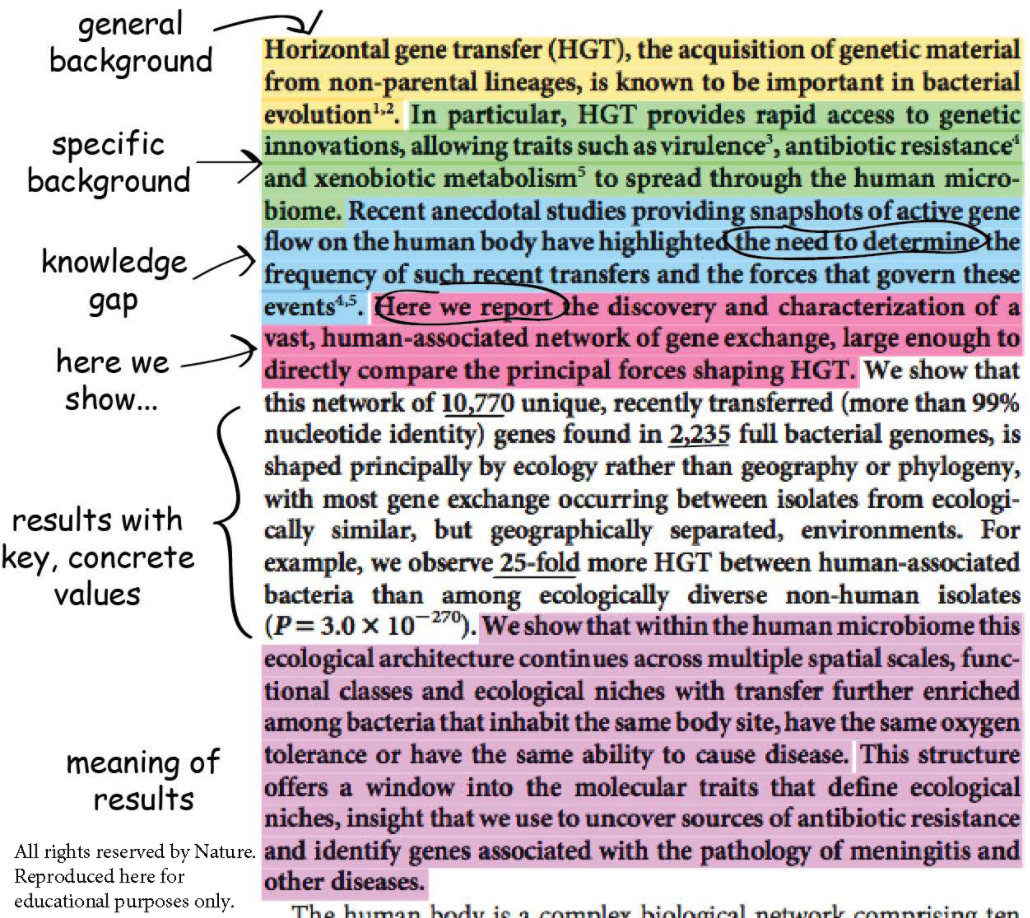
\includegraphics[width=10cm,height=10cm]{img/good-abstract.png}

%\afterpage{\blankpage}


\afterpreface





%%%%%%%%%%%%%%%%%%%%%%%%%%%%%%%%%%%%%%%%%%%%%%%%%%%%%%%%%%%%%%%%%%
%
% Now we can start on the first chapter
% Within chapters we have sections, subsections and so forth
%
%%%%%%%%%%%%%%%%%%%%%%%%%%%%%%%%%%%%%%%%%%%%%%%%%%%%%%%%%%%%%%%%%%



%%%%%%%%%%%%%%%%%%%%%%%%%%%%%%%%%%%%%

%\afterpage{\blankpage}


\hypertarget{introduction}{%
\chapter{Introduction}\label{introduction}}

Notre travail pour ce semestre consistait à créer des modèles de machine learning en utilisant un jeu de données que l’on pouvait choisir.
Nous avons choisi comme thématique les jeux vidéos, et plus précisément \textbf{la prédiction de ventes des jeux vidéos}. Ce choix de thématiques fut une
évidence pour notre groupe étant donné que nous avions déjà travaillé sur les jeux vidéo au semestre précédent en créant un site de recommandation interactif.
Ainsi, notre projet travaillé tout au long de ce module est en quelque sorte une continuité de notre travail.

Voulant travailler sur les jeux vidéos,
nous avons décidé de créer \textbf{un algorithme de machine learning afin d’estimer le nombre de ventes qu’un jeu allait faire suivant ses caractéristiques}.
Nous avons pour cela dû analyser notre jeu de données d’entraînement, entraîner les modèles, et pour rendre nos modèles accessibles, \textbf{créer un site web}.
L’objectif de ce site est de créer une interface permettant aux développeurs de jeux vidéo de pouvoir estimer les ventes que ferait leur jeu vidéo.

Ce projet s’adresse principalement aux développeurs de jeux vidéo, quelque soit leurs niveaux. Notre projet combine des modèles prédictifs et une interface utilisateur
simple et accessible. Contrairement à certains outils existants souvent compliqués ou peu accessibles.
\textbf{Notre site permet alors une estimation rapide des ventes à partir de caractéristiques basiques et facilement modifiables}.

La vidéo de soutenance est accessible ici : \url{<URL\_VIDEO\_SOUTENANCE>}.

De plus, comme nous avons rencontré des difficultés avec InfinityFree, une certaine limite d’accès quotidienne gratuite, une démonstration de notre site web
est disponible à l’adresse suivante : \url{<URL\_VIDEO\_DEMO>}. Ce rapport est organisé de la façon suivante : tout d’abord, nous présenterons les
données utilisées et leur traitement. Ensuite, nous détaillerons les modèles de machine learning utilisés ainsi que leurs performances. Enfin,
nous verrons la réalisation du site web.


%%%%%%%%%%%%%%%%%%%%%%%%%%%%%%%%%%%%%
\hypertarget{Gestion-de-projet}{%
\chapter{Gestion de projet }\label{chapGestionProjet}}

\hypertarget{IntroductionGestionProjet}{%
\section{Introduction}\label{IntroGestionProjet}}

Pour ce travail de groupe nous avons utiliser les outils Git, Github et Discord pour
unr meilleure collaboration.

Le lien vers le Github est le suivant : \url{https://github.com/Caquite/GamesSales} \\

Dans cette section nous allons parler de collaboration. Nous allons commencer par évoquer les
façon dont nous avons utiliser Git, puis nous verons les contricutions de chancun.


\hypertarget{collaborationGit}{%
\section{Collaboration avec Git}\label{collaborationGit}}

L'utilisation de Git s'est faite naturellement. Chaque participante du projet GamesSales avait assisté au cours TE5PR1MI - Gestion de projet du semestre 5.
Ainsi, nous avions toutes connaissance des bases du fonctionnement de Git. Certaines ont décidé de créer des branches afin d’avancer sur leurs parties et de vérifier
leur bon fonctionnement avant de les intégrer dans la branche principale. \textbf{L’utilisation de branches} a également été faite lorsque plusieurs tâches étaient réalisées
 \textbf{simultanément}, afin d’éviter les conflits.

Par ailleurs, seuls deux à trois conflits ont été rencontrés. Pour chacun d’eux, nous avons utilisé les outils
proposés par notre environnement de développement pour les corriger, notamment l'outil "Visual Studio Code".

Nous n’avons pas eu recours à l’historique des commits.

\hypertarget{contributionParEtudiant}{%
\section{Contribution}\label{contributionParEtudiant}}

\begin{table}[H]
\centering
\begin{tabular}{|l|c|c|c|c|}
\hline
\textbf{Tâche} & \textbf{Donia} & \textbf{Clémentine} & \textbf{Ica} & \textbf{Catherine} \\
\hline
Recherche des datasets & 25\% & 25\% & 25\% & 25\% \\
\hline
Modélisation (MCD/MOD) & 20\% & 70\% & 5\% & 5\% \\
\hline
Nettoyage des données & 5\% & 45\% & 45\% & 5\% \\
\hline
Analyse exploratoire & 25\% & 25\% & 25\% & 25\% \\
\hline
Modélisation ML & 5\% & 35\% & 25\% & 35\% \\
\hline
API Flask & 70\% & 5\% & 5\% & 20\% \\
\hline
Site web (frontend/backend) & 70\% & 10\% & 5\% & 15\% \\
\hline
Rédaction rapport & 25\% & 25\% & 25\% & 25\% \\
\hline
\end{tabular}
\caption{Répartition des contributions par tâche}
\end{table}


\begin{table}[H]
\centering
\begin{tabular}{|l|c|c|c|c|}
\hline
\textbf{Page} & \textbf{Donia} & \textbf{Clémentine} & \textbf{Ica} & \textbf{Catherine} \\
\hline
choix\_dev & 85\% & 5\% & 5\% & 5\% \\
\hline
documentation & 30\% & 5\% & 5\% & 60\% \\
\hline
index & 80\% & 5\% & 10\% & 5\% \\
\hline
prediction & 80\% & 10\% & 5\% & 5\% \\
\hline
\end{tabular}
\caption{Répartition des contributions par page}
\end{table}

Concernant les contributions visibles sur GitHub, \textbf{il est important de noter que celles-ci ne reflètent pas entièrement le travail réalisé par chaque membre du groupe}.
En effet, bien que certaines modifications aient été effectuées via des commits Git, \textbf{une partie du travail a été réalisée en dehors de la plateforme}.
Certains fichiers ont été ajoutés manuellement sur le Github et non pas en utilisant les commits. Cette façon de procédé n'a donc pas pu être pris en compte par Github.
pourtant, cela représente une partie assez importante de la conception du projet.

Nous avons également échangé des fichiers en amont, via des outils de communication tels que Discord, afin de faciliter les retours rapides et les corrections collaboratives.
Dans ces cas, un seul membre se chargeait ensuite de déposer la version finale sur GitHub, ce qui explique que certaines contributions apparaissent comme
étant réalisées par une seule personne, alors que ce n'était pas le cas. C'est pour des raisons d’efficacité et de réactivité que nous avions utiliser cette méthode par moment.
Cela nous a alors permis de gagner du temps tout au long du projet.

Ainsi, \textbf{le nombre de commits par utilisateur n'est pas un indicateur de l’implication de chacun} dans ce projet, l’ensemble du travail a été réalisé de manière
collaborative.

\hypertarget{planning}{%
\section{Planning}\label{Planning}}

ON A BESOIN DE CETTE MERDE ??????????!!!!!!!!!!!!!
POUR MOI NON ON SUPPRIME VOILA NIQUEZ TOUT LES ENSEIGNANTS LEURS CHIENS ET LEURS GROUPE DE POP PREFERE !!!!!!

AAAAAAAAAAAAAAAAAAAAAAAAAAAAAAAAAAAAAAAAAAAAAAAAAAAAAAAAAAAAAAAAAAAAAAAAAAAAAAAAAAAAAAAAAAAAAAAAAAAAAAAAAAAAAAAAAAAAAAAAAAAAAAAAAAAAAAAAAAAAAAAAAAAAAAAAAAAAAAAAAAAAAAAAAAAA
AAAAAAAAAAAAAAAAAAAAAAAAAAAAAAAAAAAAAAAAAAAAAAAAAAAAAAAAAAAAAAAAAAAAAAAAAAAAAAAAAAAAAAAAAAAAAAAAAAAAAAAAAAAAAAAAAAAAAAAAAAAAAAAAAAAAAAAAAAAAAAA
AAAAAAAAAAAAAAAAAAAAAAAAAAAAAAAAAAAAAAAAAAAAAAAAAAAAAAAAAAAAAAAAAAAAAAAAAAAAAAAAAAAAAAAAAAAAAAAAAAAAAAAAAAAAAAAAAAAAAAAAAAAAAAAAAAAAAAAAAAAAAAAAAAAAAAAAAAAAAA
AAAAAAAAAAAAAAAAAAAAAAAAAAAAAAAAAAAAAAAAAAAAAAAAAAAAAAAAAAAAAAAAAAAAAAAAAAAAAAAAAAAAAAAAAAAAAAAAAAAAAAAAAAAAAAAAAAAAAAAAAAAAAAAAAAAAAAAAAAAAAAAAAAAAAAAAAAAAAA

ce qui était écrit avant que je remplace par ce qu'il y a au dessus :

Le planning de janvier n’est surement pas celui qui a été suivi ce semestre. Indiquer les deux (l’ancien et le planning mis à jour).

Il faut donc expliquer pourquoi certaines taches ont été plus rapides ou lentes que prévu.  Comment vous vous êtes adaptés ? 


\hypertarget{ConclusionGestionProjet}{%
\section{Conclusions}\label{ConcluGestionProjet}}

AAAAAAAAAAAAAAAAAAAAAAAAAAAAAAAAAAAAAAAAAAAAAAAAAAAAAAAAAAAAAAAAAAAAAAAAAAAAAAAAAAAAAAAAAAAAAAAAAAAAAAAAAAAAAAAAAAAAAAAAAAAAAAAAAAAAAAAAAAAAAAAAAAAAAAAAAAAAAAAAAAAAAAAAAAAA
AAAAAAAAAAAAAAAAAAAAAAAAAAAAAAAAAAAAAAAAAAAAAAAAAAAAAAAAAAAAAAAAAAAAAAAAAAAAAAAAAAAAAAAAAAAAAAAAAAAAAAAAAAAAAAAAAAAAAAAAAAAAAAAAAAAAAAAAAAAAAAA
AAAAAAAAAAAAAAAAAAAAAAAAAAAAAAAAAAAAAAAAAAAAAAAAAAAAAAAAAAAAAAAAAAAAAAAAAAAAAAAAAAAAAAAAAAAAAAAAAAAAAAAAAAAAAAAAAAAAAAAAAAAAAAAAAAAAAAAAAAAAAAAAAAAAAAAAAAAAAA
AAAAAAAAAAAAAAAAAAAAAAAAAAAAAAAAAAAAAAAAAAAAAAAAAAAAAAAAAAAAAAAAAAAAAAAAAAAAAAAAAAAAAAAAAAAAAAAAAAAAAAAAAAAAAAAAAAAAAAAAAAAAAAAAAAAAAAAAAAAAAAAAAAAAAAAAAAAAAA

%%%%%%%%%%%%%%%%%%%%%%%%%%%%%%%%%%%%%

\hypertarget{BD}{%
\chapter{Base de données}\label{chapBD}}


\hypertarget{IntroductionBD}{%
\section{Introduction}\label{IntroBD}}

Afin de créer notre base de données, nous avons utilisé deux datasets trouvées sur Kaggle :

- Videogamesales : \url{https://www.kaggle.com/datasets/gregorut/videogamesales}

Liste de jeux vidéo dont les ventes dépassent 100 000 exemplaires.

- Steam store games : \url{https://www.kaggle.com/datasets/nikdavis/steam-store-games}


Informations sur les différents aspects des jeux en magasin, comme leur genre et le nombre estimé de propriétaires. \\

Voici les informations relatives aux datasets :


\begin{table}[H]
\centering
\begin{tabular}{|l|c|c|}
\hline
\textbf{Tâche} & \textbf{Videogamesales} & \textbf{Steam store games} \\
\hline
Description & 11 & 409 \\
\hline
Taille & 1325ko & 246 134ko \\
\hline
Format & .csv & .csv \\
\hline
Nombre de fichier & 1 & 6 \\
\hline
Nombre de ligne & 16 599 & 27 000 \\
\hline
Nombre de colonne & 11 & 409 \\
\hline
\end{tabular}
\caption{Informations supplémentaires sur les datasets}
\end{table}


AAAAAAAAAAAAAAAAAAAAAAAAAAAAAAAAAAAAAAAAAAAAAAAAAAAAAAAAAAAAAAAAAAAAAAAAAAAAAAAAAAAAAAAAAAAAAAAAAAAAAAAAAAAAAAAAAAAAAAAAAAAAAAAAAA
AAAAAAAAAAAAAAAAAAAAAAAAAAAAAAAAAAAAAAAAAAAAAAAAAAAAAAAAAAAAAAAAAAAAAAAAAAAAAAAAAAAAAAAAAAAAAAAAAAAAAAAAAAAAAAAAAAAAAAAAAAAAAAAAAAAAAAAAAAAAAAA
AAAAAAAAAAAAAAAAAAAAAAAAAAAAAAAAAAAAAAAAAAAAAAAAAAAAAAAAAAAAAAAAAAAAAAAAAAAAAAAAAAAAAAAAAAAAAAAAAAAAAAAAAAAAAAAAAAAAAAAAAAAAAAAAAAAAAAAAAAAAAAAAAAAAAAAAAAAAAA
AAAAAAAAAAAAAAAAAAAAAAAAAAAAAAAAAAAAAAAAAAAA

Vous introduirez ici le chapitre et donnerez le ou les url des sites sur lesquels vous avez récupéré des données.
 
  Dans les jeux de données récupérés, expliquer pourquoi vous avez
  sélectionné certaines tables. Vous devez indiquer
  comment les données sont stockées (le format), la taille des fichiers,
  le nombre, \ldots{}
  
  Donner le plan de la section.


\hypertarget{descriptifTraitementBD}{%
\section{Traitements réalisés}\label{traitementBD}}

Vous décrirez ici les étapes réalisées pour pré-traiter vos données. Expliquer quels choix vous avez réalisés pour filtrer les lignes et
  les colonnes (éventuellement réduire le périmètre du projet) et
  décrire les critères de sélection (e.g., ne garder que 5 colonnes sur
  les 15, ne garder que les lignes qui correspondent à une ville en
  particulier, \ldots).

 Préciser les nettoyages réalisés avant l'import comme l'uniformisation
  des valeurs des champs (\emph{e.g.}, Mr, M., Monsieur, \ldots) ou le
  remplissage des valeurs manquantes par une valeur moyenne \ldots{}

\hypertarget{descriptif-des-tables}{%
\section{Descriptif des tables}\label{descriptif-des-tables}}

Pour chaque table conservée, préciser le nombre de lignes et de
  colonnes après filtrage, lister les colonnes et donner pour chacune le
  type, la signification du champ et des caractéristiques (unique, clés,
  valeur manquante, \ldots) en remplissant le tableau ci-dessous.

\begin{longtable}[]{@{}cccc@{}}
\caption{Nom de la table (nombre de lignes \(\times\) nombre de
colonnes)}\tabularnewline
\toprule
Nom colonne & Type & Signification & Caractéristique \\
\midrule
\endfirsthead
\toprule
Nom colonne & Type & Signification & Caractéristique \\
\midrule
\endhead
& & & \\
\bottomrule
\end{longtable}

\hypertarget{MCD}{%
\section{Modèle conceptuel des données}\label{mcd}}

Nous avons ensuite utilisé le logiciel Mocodo pour faire un MOD et MCD de nos données dans le but de mieux comprendre leur stucture et leurs relations.

  \begin{figure}
  \hypertarget{MCD}{%
  \centering
  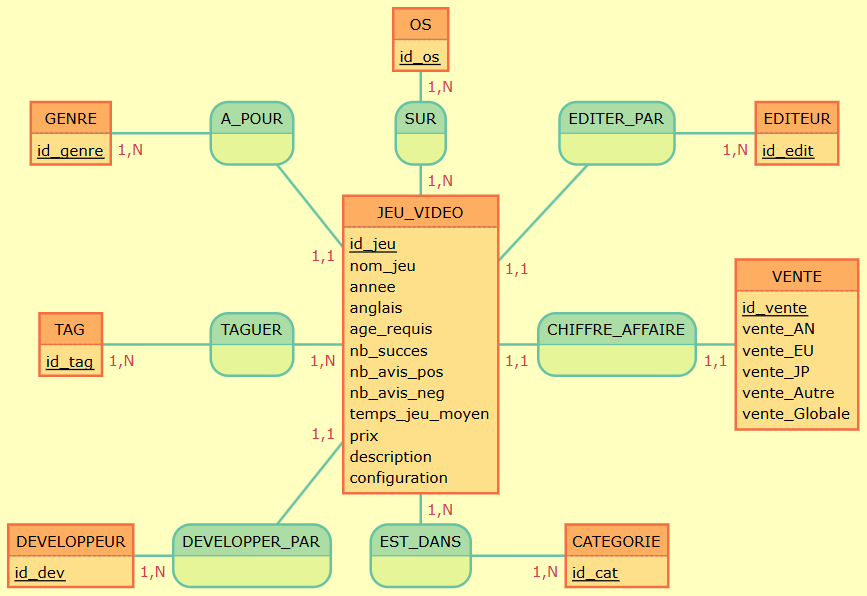
\includegraphics[width=12cm,height=8cm]{img/MCD.png}
  \caption{MCD GamesSales.}\label{MCD}
  }
  \end{figure}
  
  
\hypertarget{MOD}{%
\section{Modèle organisationnel des données}\label{mod}}

  Pour le MOD, inclure une image réalisée avec le designer de phpmyadmin
  
  SAUF QUE MOD MAL FAIT ?? OU JUSTE MOI RIEN COMPRIS ????


\hypertarget{requuxeates-ruxe9alisuxe9es}{%
\section{Requêtes réalisées}\label{requuxeates-ruxe9alisuxe9es}}

Pour les requêtes importantes dans votre interface, les exprimer en langage naturel puis en SQL. Puis
donner le résultat obtenu (ou un extrait) et expliquer ce résultat.


\hypertarget{concluBD}{%
\section{Conclusions}\label{concluBD}}

Préciser la durée de la mise en place de la BD et les  principales difficultés rencontrées.

\normalsize


%%%%%%%%%%%%%%%%%%%%%%%%%%%%%%%%%%%%%
%%%%%%%%%%%%%%%%%%%%%%%%%%%%%%%%%%%%%
\hypertarget{Analyse-exploratoire-des-données}{%
\chapter{Analyse exploratoire des données}\label{AnalyseExploratoireDesDonnées}}

\hypertarget{IntroductionAnalyseExploratoireDesDonnées}{%
\section{Introduction}\label{IntroAnalyseExploratoireDesDonnées}}

Afin de mieux appréhender les graphes les plus importants à vous présenter, nous avons réalisé cette heatmap nous indiquant la corrélation entre les différentes variables. Plus les cases sont rouges, plus il existe une forte corrélation entre les variables. Une constatation intéressante et évidente concerne la corrélation entre les trois ``types'' de ventes entre \texttt{Ventes\_AN}, \texttt{Ventes\_EU} et \texttt{Ventes\_Autre} avec la variable \texttt{Ventes\_globales}. Cependant, l’indépendance de la variable \texttt{Ventes\_JP} avec ces autres variables est tout à fait inattendue. 

Mis à part ces constatations évidentes concernant les prix, il existe aussi une corrélation entre le nombre d’avis positifs et négatifs. De plus, nous pouvons aussi remarquer que la variable concernant le nombre d’avis négatifs a plus d’impact sur le nombre de ventes que la variable concernant le nombre d’avis positif. Cela peut refléter d’une certaine manière une tendance sociétale à faire davantage remarquer les points négatifs contrairement aux points positifs.


\hypertarget{DistributionDesVentes}{%
\section{Distribution des ventes}\label{DistributionDesVentes}}

  \begin{figure}
  \hypertarget{distributionVentes}{%
  \centering
  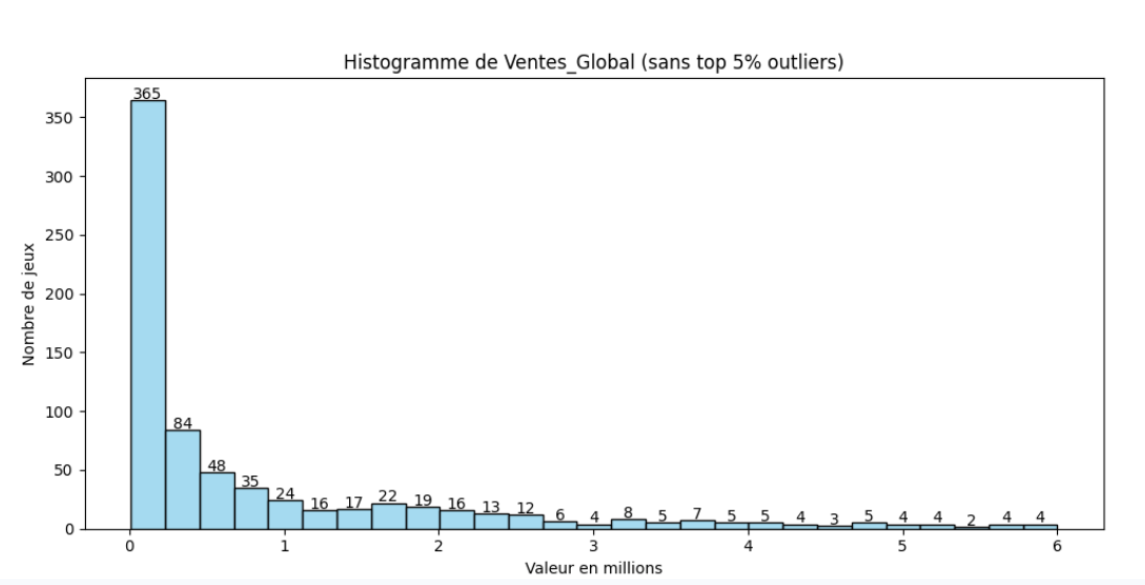
\includegraphics[width=12cm,height=8cm]{img/distributionVentes.png}
  \caption{distributionVentes GamesSales.}\label{distributionVentes}
  }
  \end{figure}

Comme premier graphique à vous présenter, nous avons choisi cet histogramme. Il représente la relation entre le nombre de ventes et le nombre de jeux. Ici il est assez rapide de se rendre compte que la majeure partie des jeux présents constituant notre base de données ont été vendu en moins d’un million d’exemplaires (environ 70\%). Sur ce graphique nous avons aussi décidé de ne pas représenter les valeurs dites aberrantes afin d'améliorer la visibilité. Cette représentation de la dispersion de nos données nous a dès cet instant mis sur la route de proposer un modèle de prédiction qui s'orienterait vers des développeurs plutôt novices ou intermédiaires.


\hypertarget{CorrélationsEntreVariables}{%
\section{Corrélations entre variables}\label{CorrélationsEntreVariables}}

  \begin{figure}
  \hypertarget{heatmap}{%
  \centering
  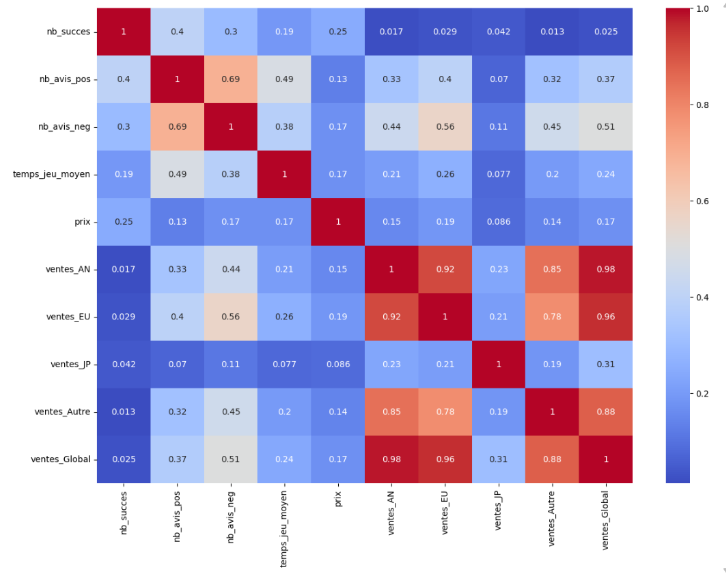
\includegraphics[width=12cm,height=8cm]{img/heatmap.png}
  \caption{heatmap GamesSales.}\label{heatmap}
  }
  \end{figure}
  
Afin de mieux appréhender les graphes les plus importants à vous présenter, nous avons réalisé cette heatmap nous indiquant la corrélation entre les différentes variables. Plus les cases sont rouges, plus il existe une forte corrélation entre les variables. Une constatation intéressante et évidente concerne la corrélation entre les trois ``types'' de ventes entre \texttt{Ventes\_AN}, \texttt{Ventes\_EU} et \texttt{Ventes\_Autre} avec la variable \texttt{Ventes\_globales}. Cependant, l’indépendance de la variable \texttt{Ventes\_JP} avec ces autres variables est tout à fait inattendue. 

Mis à part ces constatations évidentes concernant les prix, il existe aussi une corrélation entre le nombre d’avis positifs et négatifs. De plus, nous pouvons aussi remarquer que la variable concernant le nombre d’avis négatifs a plus d’impact sur le nombre de ventes que la variable concernant le nombre d’avis positif. Cela peut refléter d’une certaine manière une tendance sociétale à faire davantage remarquer les points négatifs contrairement aux points positifs.


\hypertarget{RelationVentesEtAvis}{%
\section{Relation ventes et avis}\label{RelationVentesEtAvis}}

  \begin{figure}
  \hypertarget{ventesAvis}{%
  \centering
  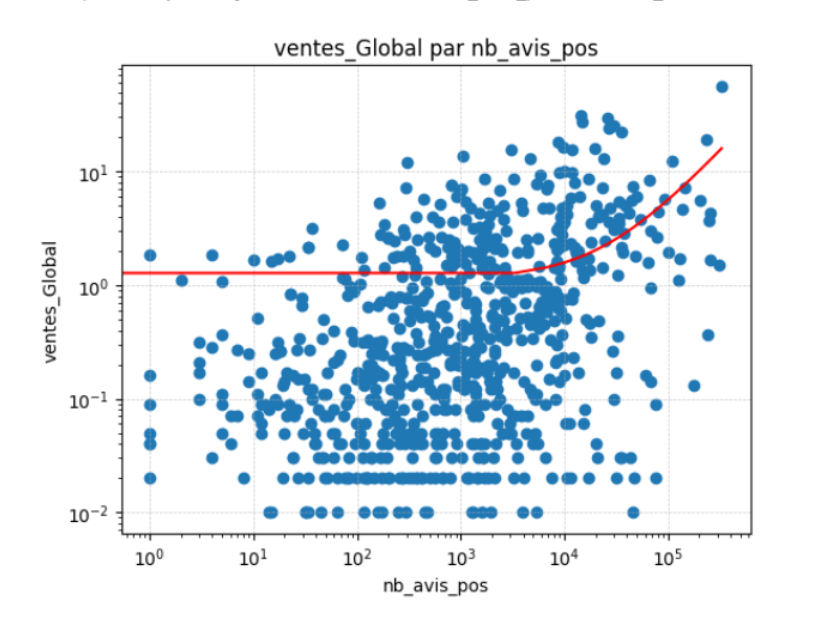
\includegraphics[width=12cm,height=8cm]{img/ventesAvis.png}
  \caption{ventesAvis GamesSales.}\label{ventesAvis}
  }
  \end{figure}
  
  
Nous avons cependant tout de même décidé de vous montrer ce nuage de point (à l'échelle logarithmique) concernant la corrélation entre le nombre de ventes et le nombre d’avis positif. Nous avons, pour compléter ce graphique calculé le coefficient de corrélation qui nous indique que la droite obtenue explique seulement  13.39\% des données. De plus, nous avons calculé la p-value : avec 5\% de risques de se tromper , nous devons rejeter l’hypothèse induisant que les deux variables soient corrélées.


\hypertarget{AnalyseDesVentesParGenre}{%
\section{Analyse des ventes par genre}\label{AnalyseDesVentesParGenre}}

  \begin{figure}
  \hypertarget{ventesGenre}{%
  \centering
  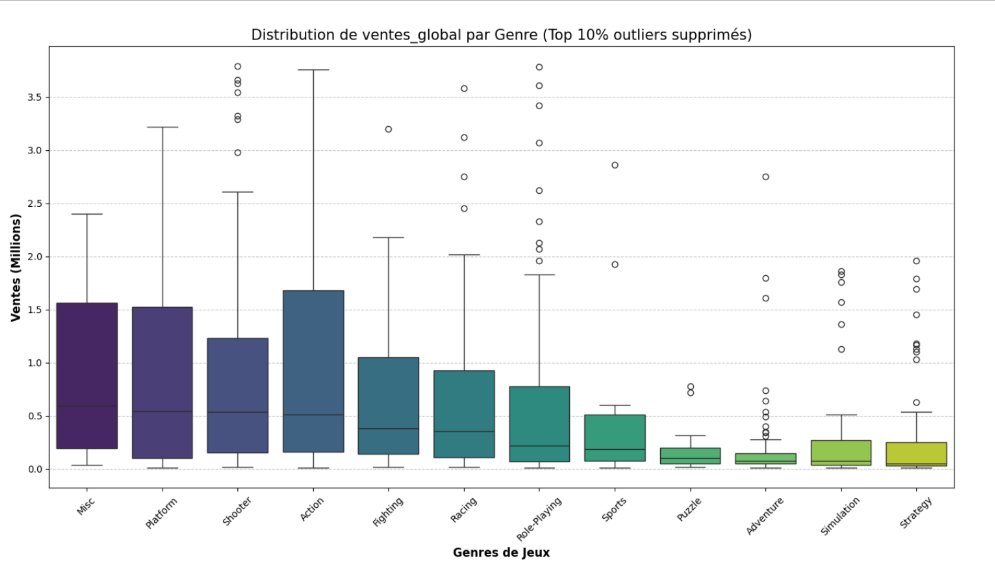
\includegraphics[width=12cm,height=8cm]{img/ventesGenre.png}
  \caption{ventesGenre GamesSales.}\label{ventesGenre}
  }
  \end{figure}
  

Avec ces premiers box-plots représentant les ventes des jeux vidéos selon leur genre, nous pouvons très rapidement penser qu’il existe une corrélation entre ces deux variables. En effet, nous pouvons constater que les genres Puzzle, Adventure, Simulation, et Strategy sont moins vendus en un nombre d’exemplaire plus restreint. A contrario, les genres Action, Platform, Misc ont l’air de se vendre plus facilement, ou du moins en plus grand nombre. Il sera intéressant de comparer ces résultats avec le diagramme en mosaïque que l’on vous présentera plus tard et qui indiquera la proportion de jeux sortis par année selon leur genre.


\hypertarget{AnalyseDesVentesParAnnée}{%
\section{Analyse des ventes par année}\label{AnalyseDesVentesParAnnée}}

  \begin{figure}
  \hypertarget{ventesAnnee}{%
  \centering
  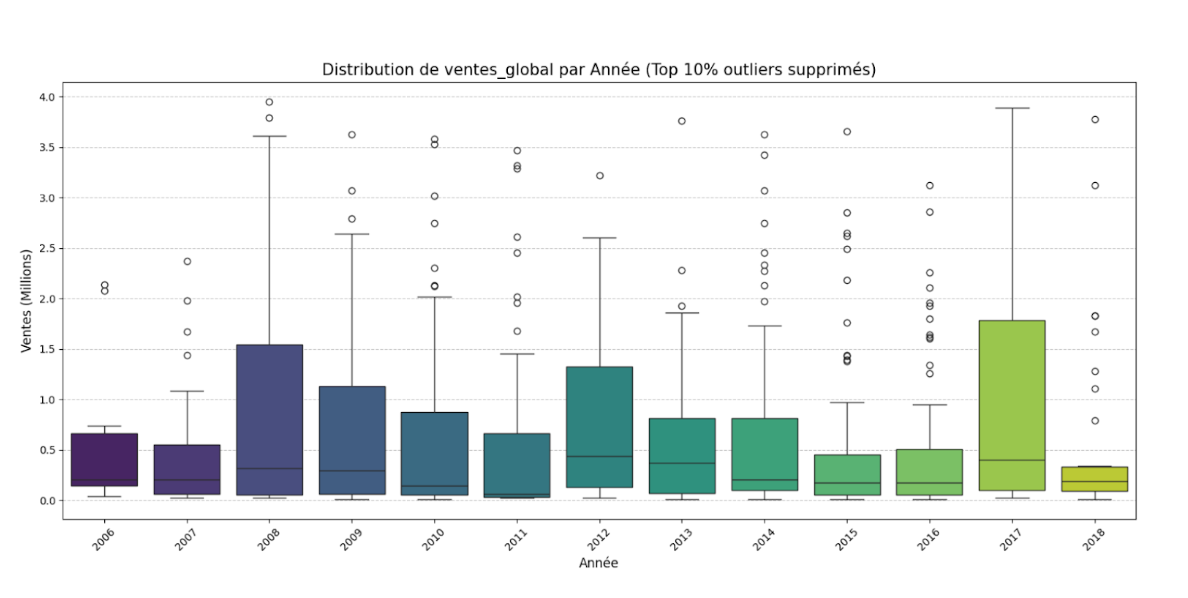
\includegraphics[width=12cm,height=8cm]{img/ventesAnnee.png}
  \caption{ventesAnnee GamesSales.}\label{ventesAnnee}
  }
  \end{figure}
  
  
Par ce box-plot, nous souhaitions étudier la répartition des ventes des jeux vidéo suivant leur année de sortie. Tout d’abord nous savons ainsi que les jeux constituant notre base de données sont sortis entre 2008 et 2018. Ce graphique révèle une globale stabilité dans le nombre de ventes jusqu’en 2015. Cependant, durant l’année 2017 le nombre de ventes a fortement augmenté en devenant l’année avec le plus de ventes si l’on se base sur les quartiles et la médiane. En 2018, les données paraissent anormalement basses : c'est probablement dû au fait que nos données ne contiennent pas beaucoup de jeux sortis cette année-là, du à la suppression des valeurs aberrantes.

\hypertarget{RelationVentesEtPrixParPériode}{%
\section{Relation ventes et prix par période}\label{RelationVentesEtPrixParPériode}}

  \begin{figure}
  \hypertarget{ventesPrix}{%
  \centering
  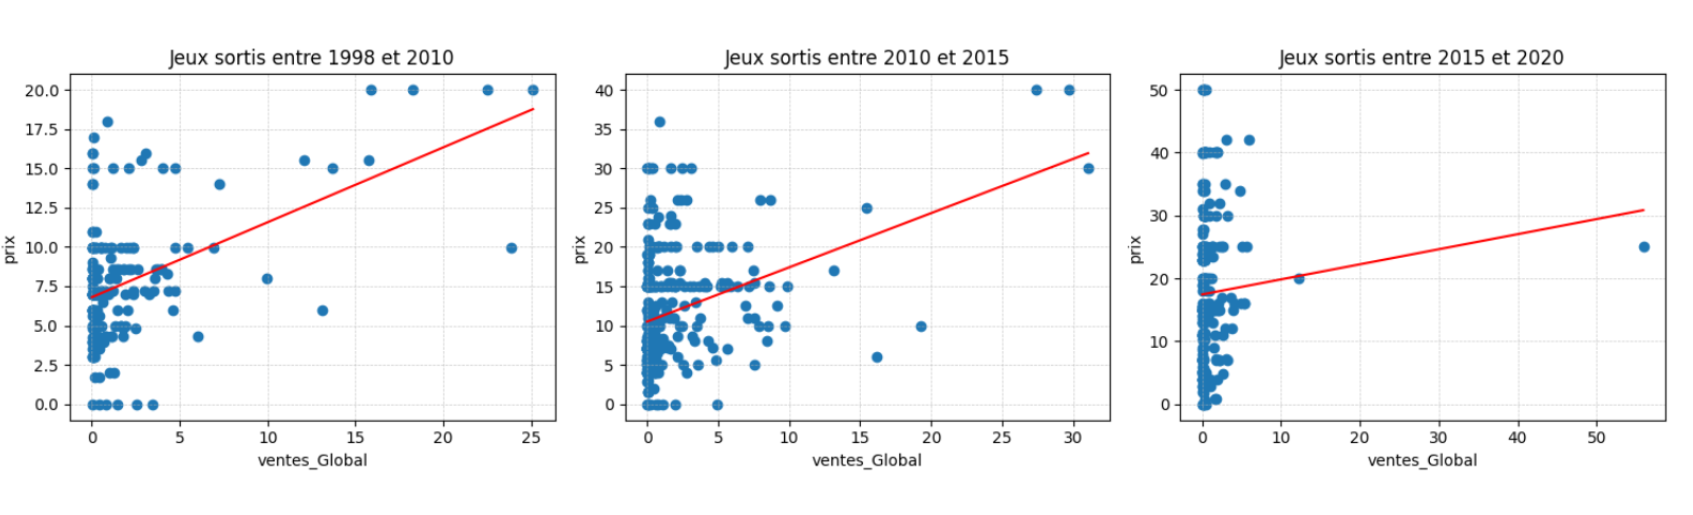
\includegraphics[width=12cm,height=8cm]{img/ventesPrix.png}
  \caption{ventesPrix GamesSales.}\label{ventesPrix}
  }
  \end{figure}
  
  
Ce graphique présente trois nuages de points illustrant la relation entre les ventes globales et les prix des jeux sortis, le tout divisé en trois périodes : 1998-2010, 2010-2015 et 2015-2020. Ce découpage a été fait afin de mieux observer l’évolution de cette relation au fil du temps.

Une première chose qui peut nous surprendre concerne la première période qui commence en 1998 pour se terminer en 2010. Si nous nous référons au graphe précédent, nos données ne débutent qu’à partir de 2008, cependant nous avions appliqué un filtre retirant les valeurs dites ``aberrantes''. Cependant, concernant ce graphique qui sépare la nos données en 3 échelles de temps nous avons jugé préférable de garder toutes nos données. 

A première vue, nos graphes semblent similaires. Cependant si nous prêtons attention aux échelles, nous pouvons très rapidement constater que la période 2010/2015 contient des jeux qui se sont vendus jusqu’à légèrement plus de 30 millions d’exemplaires et plus cher encore. Concernant la période 2015/2020, il y a moins de jeux qui se sont vendu en grand nombre d’exemplaires, cependant les jeux se vendent plus chers.

Cette fois-si, pour garder une certaine cohérence, on a choisi de ne pas utiliser d’échelle logarithmique sur l’axe des abscisses. Sinon, ça aurait rendu la comparaison des graphes côte à côte plus compliquée et moins intuitive.


\hypertarget{ÉvolutionDesGenresDansLeTemps}{%
\section{Évolution des genres dans le temps}\label{ÉvolutionDesGenresDansLeTemps}}

  \begin{figure}
  \hypertarget{mosaique}{%
  \centering
  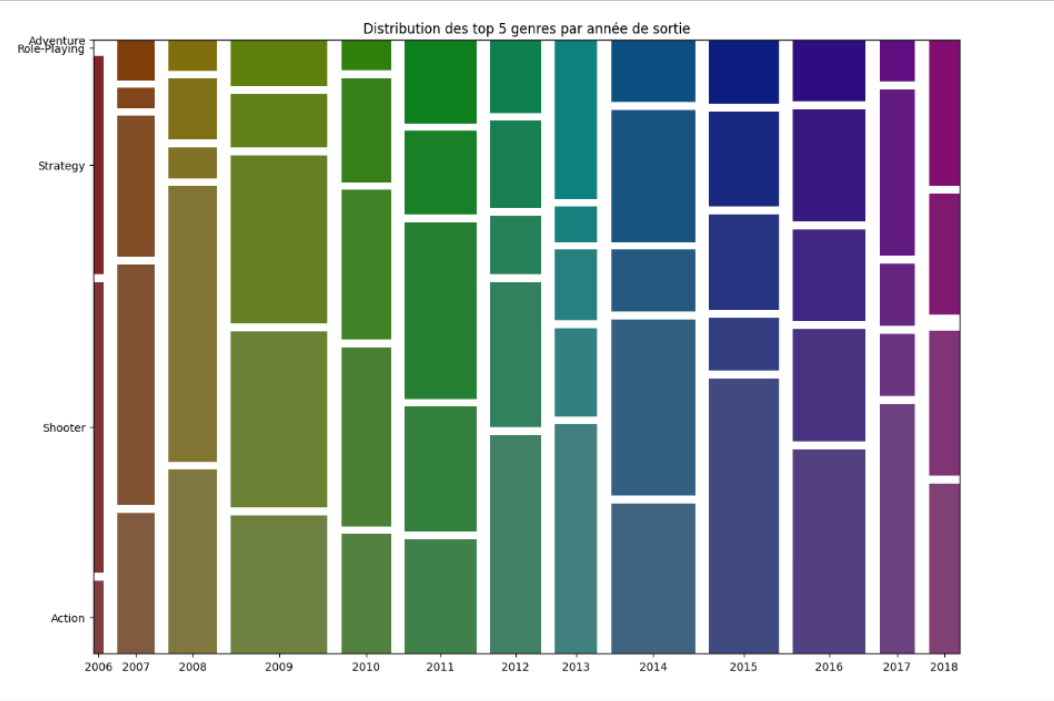
\includegraphics[width=12cm,height=8cm]{img/mosaique.png}
  \caption{mosaique GamesSales.}\label{mosaique}
  }
  \end{figure}
  
Ce graphique mosaïque illustre l'évolution de la répartition des genres au fil des années. Nous constatons qu'entre 2006 et 2010, les jeux ``Shooter'' dominaient largement notre échantillon. Cependant, à partir de 2012, la catégorie ``Action'' prend la première place jusqu'à 2018. En parallèle, les autres genres comme la stratégie ou l'aventure fluctuent de manière beaucoup plus irrégulière selon les années. Ces variations prouvent que la structure du marché change selon l'époque. Il est donc nécessaire d'associer les variables genres et année pour que notre modèle intègre cette dimension temporelle dans ses prédictions.


\hypertarget{RépartitioDesCatégories}{%
\section{Répartition des catégories}\label{RépartitioDesCatégories}}

  \begin{figure}
  \hypertarget{categories}{%
  \centering
  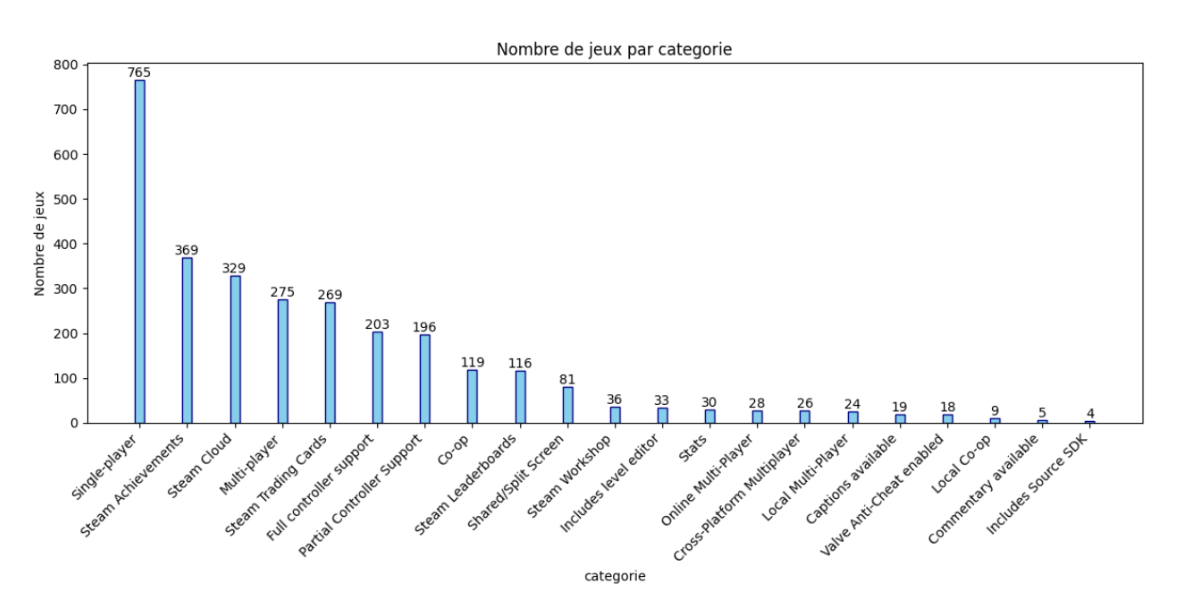
\includegraphics[width=12cm,height=8cm]{img/categories.png}
  \caption{categories GamesSales.}\label{categories}
  }
  \end{figure}
  
Ce graphique mosaïque illustre l'évolution de la répartition des genres au fil des années. Nous constatons qu'entre 2006 et 2010, les jeux ``Shooter'' dominaient largement notre échantillon. Cependant, à partir de 2012, la catégorie ``Action'' prend la première place jusqu'à 2018. En parallèle, les autres genres comme la stratégie ou l'aventure fluctuent de manière beaucoup plus irrégulière selon les années. Ces variations prouvent que la structure du marché change selon l'époque. Il est donc nécessaire d'associer les variables genres et année pour que notre modèle intègre cette dimension temporelle dans ses prédictions.


%%%%%%%%%%%%%%%%%%%%%%%%%%%%%%%%%%%%%

\hypertarget{description}{%
\chapter{Description technique et fonctionnelle}\label{description}}

\hypertarget{introDescription}{%
\section{Introduction}\label{introDescription}}


Introduire le chapitre et donner le plan de la section.


\hypertarget{Description technique}{%
\section{Description technique}\label{DescriptionT}}

Vous listerez les  technologies utilisées (Git, Php, Javascript, Mamp…) 

Vous inclurez un schéma de l’architecture de votre application


\hypertarget{Description fonctionnelle}{%
\section{Description fonctionnelle}\label{DescriptionF}}


 Par écran, 
 \begin{itemize}
 \item quelles sont les fonctionnalités, que peut faire l’utilisateur ? 
 \item quelle gestion des erreurs avez vous prévu : par exemple, sur un écran de connexion, on peut vérifier que un email contient un ‘@‘, qu’un mot de passe n’est pas trop facile..
 \end{itemize}

Ne pas hésiter à lister les fonctionnalités que vous n’avez pas eu le temps d’implémenter pour montrer que vous y avez quand même pensé. Idem pour la gestion des erreurs.

\hypertarget{concluBD}{%
\section{Conclusions}\label{concluDescription}}

Conclure et lister les difficultés rencontrées.



\hypertarget{conclusion-et-perspectives}{%
\chapter{Conclusions et perspectives}\label{conclusion-et-perspectives}}




Résumer vos contributions puis donner des perspectives à vos travaux. C est pour nous la partie importante : s’il l’on vous prenait en stage pour 2 mois sur votre sujet, auriez vous des idées et seriez vous autonomes pour améliorer votre application. 
Combien de temps auriez vous besoin pour ajouter ces fonctionnalités ? 

On attend de vous deux types de perspectives : des perspectives à court
terme pour améliorer rapidement votre approche et des perspectives à
plus long terme qu'elles soient liées à la science des données ou au
domaine métier pour lequel vous avez travaillé.



\hypertarget{annexes}{%
\chapter*{Annexes}\label{annexes}}
\addcontentsline{toc}{chapter}{Annexes}



\end{document}

